\section{Evaluation}
\label{sec:eval}

In this section, we use simulations to characterize the performance of each of our three recovery algorithms in terms of message and time overhead. 
Our goal is to illustrate the relative performance of our recovery algorithms over different topology types (e.g., \er graphs, Internet-like graphs) and
different network conditions (e.g., fixed link costs, changing link costs).
We evaluate recovery after a single compromised node has distributed false routing state.
%We count the number of messages required for nodes to find valid routing paths and count the number timesteps (epochs) for each algorithm to converge.

We build a custom simulator with a synchronous communication model: nodes send and receive messages at fixed epochs.  In each epoch, a node receives a
message from all its neighbors and performs its local computation.  In
the next epoch, the node sends a message (if needed).   All algorithms
are deterministic under this communication model.
The synchronous communication model, although simple, yields
interesting insights into the performance of each of the recovery
algorithms. Evaluation of our algorithms using a more general
asynchronous communication model is currently under
investigation. However, we believe an asynchronous implementation
will demonstrate similar trends.  

We simulate the following scenario:

\begin{enumerate}
	\item Before $t'$, $\forall v \in V$ \minvv and \dmatrixv are correctly computed.

	\item At time $t'$, \bad is compromised and advertises a \badvector (a vector with a cost of $1$ to \emph{every} node in the network) to its neighboring nodes.

	\item \badvector spreads for a specified number of hops (this varies by experiment).  Variable $k$ refers to the number of hops that \badvector has spread.

	\item At time $t$, some node $v \in V$ notifies all $v \in adj($\bads$)$ that \bad was compromised. 
	{\footnote { \small For \cpr this node also indicates the time, $t'$, \bad was compromised.}} 

\end{enumerate}
The message and time overhead are measured in step (4) above. The pre-computation common to all three recovery algorithms, described in Section \ref{subsec:preprocess},
is not counted towards message and time overhead.


\subsection{Fixed Link Weight Experiments}
\label{subsec:fixed}

In the next three experiments, we evaluate our recovery algorithms over different topology types in the case of fixed link costs.

We start with a simplified experiment setting to measure the 
 message and time overhead incurred by each of the recovery
 algorithms. In particular, we consider 
Erd\"{o}s-R\'enyi graphs with parameters $n$ and $p$. Further, the
link weight of each edge in the graph is set to 50.
$n$ is the number of graph nodes and $p$ is the probability that link $(i,j)$ exists where $i,j \in V$. We iterate over different values of $k$. For each $k$, we 
generate an Erd\"{o}s-R\'enyi graph, $G = (V,E)$, with parameters $n$ and $p$. Then we select a $v \in V$ uniformly at random and simulate the scenario described above, 
using $v$ as the compromised node. In total we sample $20$ unique nodes for each $G$.
We set $n=100$, $p=\{0.05,0.15,0.25, 0.25\}$, and let $k=\{1,2,
... 10\}$. Each data point is an average over $600$ runs ($20$ runs over 
$30$ topologies).  We then plot the $90 \%$ confidence interval.




\purge and \second message overhead increases with larger $k$. Larger $k$ implies more paths to repair, and therefore increased messaging.
For values of $k$ greater than a graph's diameter, the message overhead remains constant, as expected. 


\subsubsection{Experiment 2 - \er Graphs with Fixed but Randomly Chosen Link Weights}
\label{subsec:expt2}


The experimental setup is identical to Experiment 1 with one exception: link weights are selected uniformly at random between $[1,n]$ (rather than using 
fixed link weight of $50$).

Figure \ref{fig:msg-rand} show the message overhead for different $k$ for $p=.05$. We omit the figures for the other $p$ values because they follow the 
same trend as $p=.05$ \cite{Tech}.
In striking contrast to Experiment 1, \purge outperforms \second for all values of $k$. 
{\footnote {\small In some cases (e.g., $k=1$ for $p=.15$ and $p=.50$) \second performs better than \purges.  In these cases, \second has few routing loops \cite{Tech}.
}}
\second performs poorly because the \infinity problem: Table \ref{tab:loop1} shows the large average number of pairwise routing loops in this experiment, 
an indicator of the occurrence of \infinity problem.
No routing loops are found with \purges. \cpr performs well for the same reasons described in Section \ref{subsubsec:expt1}.  




\begin{figure*}[t]
\centering

%\subfigure[{Message overhead for \er graph with link weights selected uniformly random from $[1,100]$. $p=.05$ and diameter=$6.14$.}]{ 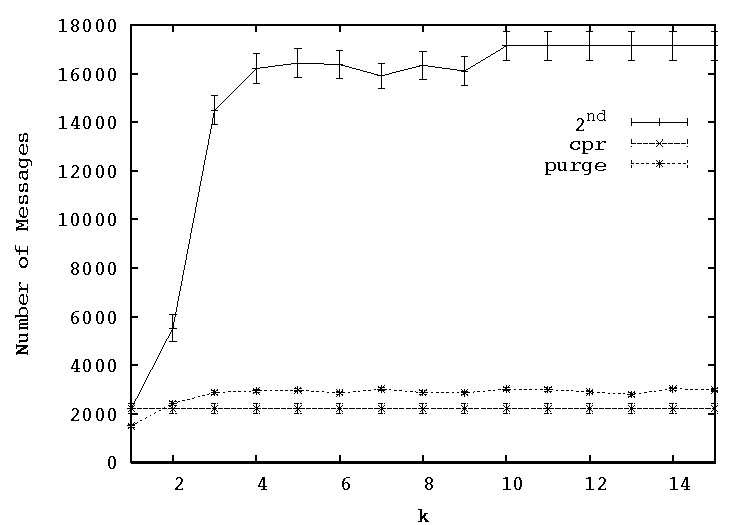
\includegraphics[scale=.35]{figs/rollback-msg-rand5.pdf}}
%\subfigure[{Message overhead for $p=0.05$ \er with link weights selected uniformly random with different $\lambda$ values. $z$ refers to the number of timesteps \cpr must rollback.}]
%	{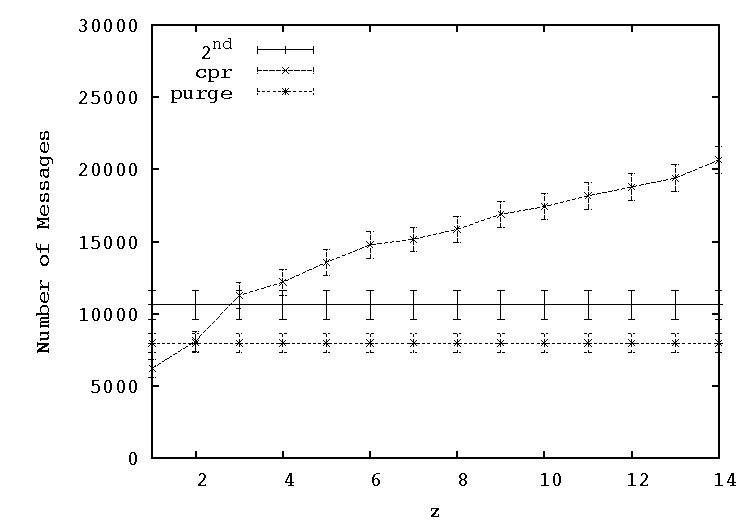
\includegraphics[scale=.35]{figs/rollback-p05-k4.pdf}} 

\subfigure[{sim 1.}]{ 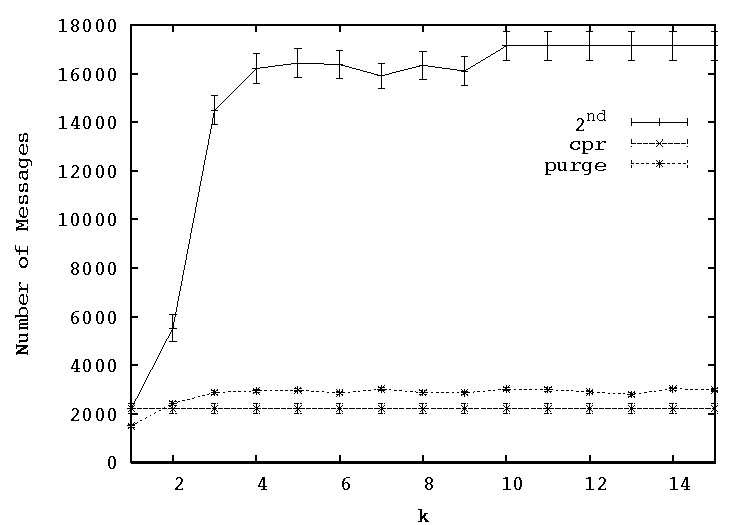
\includegraphics[scale=.55]{figs/rollback-msg-rand5.pdf}}
\subfigure[{sim 2.}] {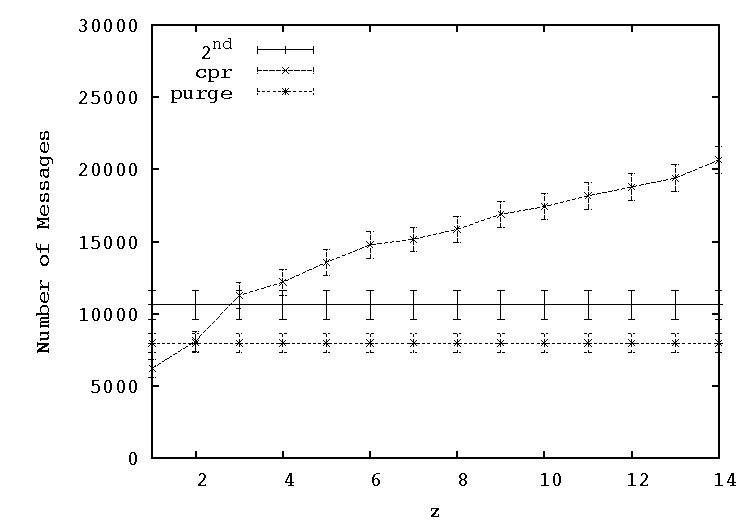
\includegraphics[scale=.55]{figs/rollback-p05-k4.pdf}} 


\caption{Rollback simulations} 
\label{fig:rollback-simulations}
\end{figure*} 


%\begin{figure}[t]
%\centering
%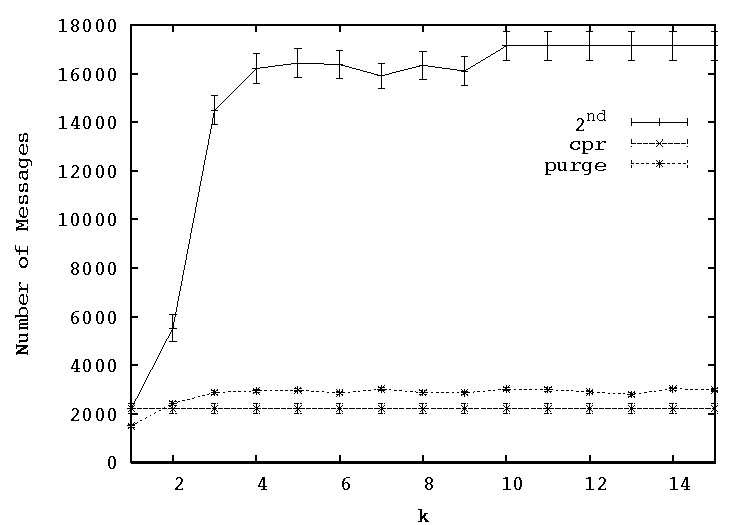
\includegraphics[scale=.35]{figs/rollback-msg-rand5.pdf}
%\caption{Message overhead for \er graph with link weights selected uniformly random from $[1,100]$. $p=.05$ and diameter=$6.14$.}
%\label{fig:msg-rand}
%\end{figure}


In addition, we counted the number of epochs in which at least one pairwise routing loop existed.  For \second (across all topologies), on average, all but the last three 
timesteps had at least one routing loop.  This suggests that the \infinity problem dominates the cost for \seconds. 




\subsection{Link Weight Change Experiments}
\label{subsec:change}

So far, we have evaluated our algorithms over different topologies with fixed link costs. We found that \cpr outperforms the other algorithms because \cpr removes false
routing state with a single diffusing computation, rather than using an iterative process like \second and \purges.  In the next 
two experiments we evaluate our algorithms over graphs with changing link costs. We introduce link cost changes between the time \bad is compromised and when \bad is discovered 
(e.g. during $[t',t]$). 
In particular, there are $\lambda$ link cost changes per timestep, where $\lambda$ is deterministic. 
To create a link cost change event, we modify links uniformly at random (except for all $(v,\bar{v})$ links). % where $v \in V'$ and $v \in adj(\bar{v})$.
The new link cost is selected uniformly at random from $[1,n]$. 


\subsubsection{Experiment 5}

In this experiment we study the trade-off between message overhead and storage overhead for \cprs. To this end, we vary the frequency at which \cpr checkpoints and fix 
the interval $[t',t]$. Otherwise, our experimental setup is the same as Experiment 4.

Due to space constraints, we only display a single plot. Figure \ref{fig:lc-fixk} shows the results for an \er graph with link weights selected uniformly at random between $[1,n]$,
$n=100$, $p=.05$, $\lambda=4$ and $k=2$. We plot message overhead against the number of timesteps \cpr must rollback, $z$. \cprs's message overhead increases with larger $z$ 
because as $z$ increases there are more link cost change events to process. \second and \purge have constant message overhead because they operate independent of $z$.

We conclude that as the frequency of \cpr snapshots decreases, \cpr incurs higher message overhead.  Therefore, when choosing the frequency of checkpoints,
the trade-off between storage and message overhead must be carefully considered. 


%\begin{figure}[t]
%\centering
%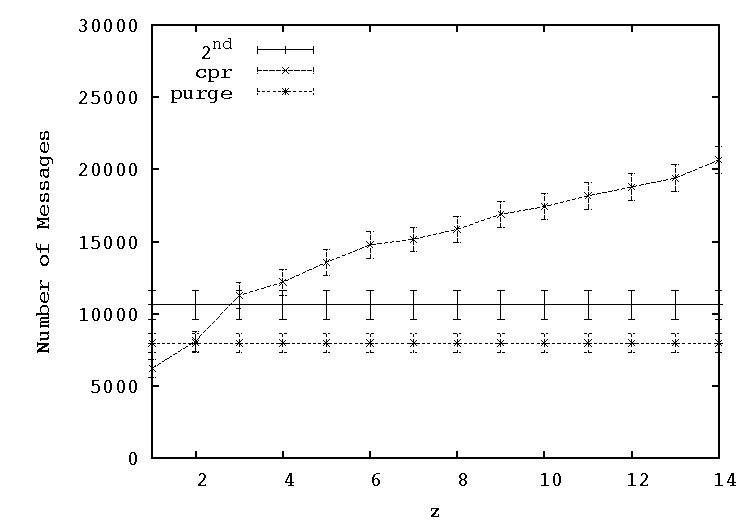
\includegraphics[scale=.35]{figs/rollback-p05-k4.pdf}
%\caption{Message overhead for $p=0.05$ \er with link weights selected uniformly random with different $\lambda$ values. $z$ refers to the number of timesteps \cpr must rollback.}
%\label{fig:lc-fixk}
%\end{figure} 






\subsection{Summary}
\label{subsec:discuss}

Our results show that for graphs with fixed link costs, \cpr yields the lowest message and time overhead. \cpr benefits from removing false state with a single
diffusing computation. However, \cpr has storage overhead, requires loosely synchronized clocks, and requires the time \bad was compromised be identified.

\seconds's performance is determined by the \infinity problem. In this case of \er graphs with fixed unit link weights, the \infinity problem was minimal, 
helping \second perform better than \purges. \purge avoids the \infinity problem by first globally invalidating false state.  Therefore in cases where the \infinity problem is 
significant, \purge outperforms \seconds.

When considering graphs with changing link costs, \cprs's performance suffers because it must process all valid link cost changes that occurred since \bad was compromised.
Meanwhile, \second and \purge make use of computations that followed the injection of false state, that do not depend on false routing state. However, \seconds's performance degrades 
because of the \infinity problem.  \purge eliminates the \infinity problem and therefore yields the best performance over topologies with changing link costs.

Finally, we found that an additional challenge with \cpr is setting the parameter which determines the checkpoint frequency.
More frequent checkpointing yields lower message and time overhead at the cost of more storage overhead. Ultimately, application-specific factors must be considered
when setting this parameter. 

